\begin{homeworkProblem}

The Curse and Blessing of Dimensionality. Denote $\boldsymbol{x}=\left(x_1, \ldots, x_d\right)$.

(a) The $d$-dimensional hyperball of radius $r$ is denoted as
$$B_d(r)=\left\{\boldsymbol{x} \in \mathbb{R}^d: \sum_{i=1}^d x_i^2 \leq r^2\right\}$$

Find the volume of $B_d(r)$ and plot a figure to show how such volume changes with $d$ when $r=1$.

(b) The $d$-dimensional hypersphere of radius $r$ is denoted as
$$S_{d-1}(r)=\left\{\boldsymbol{x} \in \mathbb{R}^d: \sum_{i=1}^d x_i^2=r^2\right\}$$
When $d \gg 1$, adopt concentration inequalities to show almost all the volume of the high-dimensional hypersphere lies near its equator.

(c) The $d$-dimensional hypercube of radius $r$ is denoted as
$$C_d(r)(r)=\left\{\boldsymbol{x} \in \mathbb{R}^d:-r \leq x_i \leq r\right\}$$
When $d \gg 1$, adopt concentration inequalities to show almost all the volume of the high-dimensional cube is located in its corners.

\solution

(a) Suppose that the $d$-dimensional hyperball with radius $r$'s volume is $V_d(r)$. We can get that
\begin{align*}
V_d(r) &= C_d(r) \cdot r^d \\
&= \int_{-r}^r C_{d-1}(r) \left(\sqrt{r^2 - x^2}\right)^{d-1} \dx \\
&= 2C_{d-1}(r) \int_0^r \left(\sqrt{r^2 - x^2}\right)^{d-1} \dx \\
&= 2 C_{d-1}(r) \int_0^{\pi / 2} r^d (\cos\theta)^{d} d\theta
\end{align*}

And we can get that
$$
C_d(r) = 2 C_{d-1}(r) \cdot \frac{(d-1)!!}{d!!} \cdot \frac{\pi}{2} \quad \text{if } d \text{ is even}
$$

$$
C_d(r) = 2 C_{d-1}(r) \cdot \frac{(d-1)!!}{d!!} \quad \text{if } d \text{ is odd}
$$

where $n!!$ is the double factorial of $n$, which is defined as $n!! = n \cdot (n-2) \cdot (n-4) \cdots 1$ if $n$ is odd, and $n!! = n \cdot (n-2) \cdot (n-4) \cdots 2$ if $n$ is even. We can get that

$$
C_d(r) = 
\begin{cases}
2 \cdot \frac{2 \pi}{3} \cdot \frac{2 \pi}{5} \cdot \cdots \cdot \frac{2 \pi}{d} & \text{if } d \text{ is odd} \\
\pi \cdot \frac{2 \pi}{4} \cdot \frac{2 \pi}{6} \cdot \cdots \cdot \frac{2 \pi}{d} & \text{if } d \text{ is even}
\end{cases}
= \frac{\pi^{\frac{d}{2}}}{\Gamma\left(\frac{d}{2} + 1\right)}
$$
So above all,
$$
V_d(r) = \frac{\pi^{\frac{d}{2}}}{\Gamma\left(\frac{d}{2} + 1\right)} \cdot r^d
$$
The voulme of the unit hyperball changes via dimension $d$ is shown in the following figure, we could discover that when $d=5$, the volume of the unit hyperball reaches its maximum value, and then it decreases as $d$ increases.

\begin{figure}[h]
    \centering
    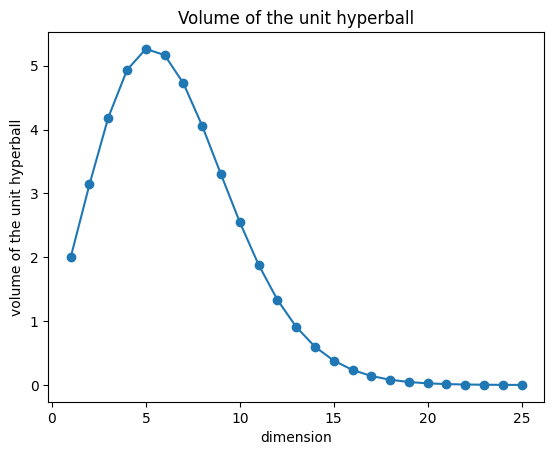
\includegraphics[width=0.6\textwidth]{./figure/p8/volume.png}
    \caption{volume of the unit hyperball}
\end{figure}


(b) Consider uniformly sampling from the hypersphere. i.e. $\boldsymbol{x}=(x_1,\ldots,x_d)$, by symmetry, we can get that $x_1,\ldots,x_d$ has the same distribution. So $\E(x_1)=\ldots=\E(x_d)=0$. Since $\boldsymbol{x}$ samples from hypersphere, so
\begin{align*}
x_1^2 + x_2^2 + \ldots + x_d^2 &= r^2 \\
\E\left(x_1^2 + \ldots + x_d^2\right) = \E(r^2) &= r^2 \\
\Var(x_d) = \E(x_d^2) &= \dfrac{r^2}{d}
\end{align*}

Let $\epsilon \ll r$, let the equator to be if $\boldsymbol{x}=\left\{(x_1,\ldots,x_d)\in S_{d-1}(r) \big| |x_d| < \epsilon\right\}$.
According to Chebyshev's Inequality:
\begin{align*}
P(|x_d - \E(x_d)| \geq \epsilon) \leq \frac{\Var(x_d)}{\epsilon^2} \\
P(|x_d| \geq \epsilon) \leq \dfrac{r^2}{d \epsilon^2}
\end{align*}



When $d$ is very large, $\dfrac{r^2}{d \epsilon^2} $ becomes extremely small.
Thus, it becomes highly unlikely that the sampled data will be a point where $ |x_d| \geq \epsilon $.
In other words, the sampled data is almost certainly located near the equator.
Since the sampling is uniform over the hypersphere,
we can conclude that nearly all the volume of a high-dimensional hypersphere is concentrated near its equator.


When the dimension $d\gg 1$, $\dfrac{r^2}{d \epsilon^2}\to 0$, which means it's very unlikely to pick a point where $|x_d| \geq \epsilon$. i.e. most points end up being near the equator. And since the points are sampled uniformly, it tells us that almost all of the hypersphere's volume in high dimensions is concentrated near its equator.


(c) The volume of the cube is $(2r)^d$. Let $x_1, x_2, \dots, x_d\stackrel{i.i.d.}{\sim}\Unif(-r, r)$. So $\Var(x_i) = \dfrac{r^2}{3}$.

With the Chebyshev's Inequality, we can get that $\forall t > 0$:
$$P\left( \sum_{i=1}^d x_i^2 \leq r^2 \right) \leq e^{t r^2} \left( \mathbb{E}(e^{-t x_1^2}) \right)^d$$
Take $t=1$, we have:
$$\mathbb{E}\left(e^{-x_1^2}\right) = \int_{-r}^{r} \frac{1}{2r} e^{-x_1^2} \dx_1 < \int_{-r}^{r} \frac{1}{2r} \dx_1 = 1$$

Thus, $\mathbb{E}^d\left(e^{-x_1^2}\right)\to 0$ as $d$ increases, i.e.
$$\lim_{d \to \infty} P\left( \sum_{i=1}^d x_i^2 \leq r^2 \right) = 0$$
It is nearly impossible to sample a point from the hyperball insiede the hypercube, nearly all of the volume of the high-dimensional cube is concentrated near its corners.

\end{homeworkProblem}

\newpage